\chapter{Podsumowanie}
\label{cha:podsumowanie}


%---------------------------------------------------------------------------

\section{Podsumowanie i wnioski}
\label{sec:podsumowanieIWnioski}

Celem pracy było zaprojektowanie, implementacja i ewaluacja mechanizmu pozyskiwania wiedzy o  stanie emocjonalnym użytkownika w systemach \textit{affective computing}.  

Na potrzeby pracy zaprojektowana i zaimplementowana została aplikacja mobilna pozwalająca na uczynienie jawnej mediacji wiedzy możliwie nieintruzywną (poprzez wnioskowanie oparte na monitorowaniu czynników zewnętrznych) oraz na przeprowadzenie niejawnej mediacji (z wykorzystaniem aparatu fotograficznego telefonu). 

Cel udało się zrealizować, a potwierdzeniem tego są wyniki ewaluacji z poprzedniego rozdziału. Badanie wśród grona użytkowników potwierdziło, że stworzona aplikacja spełniła swoje podstawowe założenia, przede wszystkim czyniąc proces mediacji wiedzy bardziej skutecznym i przyjaznym dla uczestnika badania.

Podczas realizacji pracy wyprowadzono następujące wnioski:

\begin{itemize}
	\item Odczytywanie emocji przez urządzenia może przyczynić się do polepszenia jakości życia w kategoriach: rozrywki, nauki, pracy, marketingu, bezpieczeństwa i wielu innych.
	
	\item Smartfon, jako urządzenie, które zawsze jest pod ręką, nadaje się bardzo dobrze do monitorowania nastroju użytkownika.
	
	\item Na dłuższą metę nagrywanie dźwięku, robienie zdjęć, czy odpytywanie użytkownika nie ma racji bytu z uwagi na naturalną dla człowieka potrzebę chronienia swojej prywatności. Konieczne jest wprowadzenie nowych metod rozpoznawania nastroju, najlepiej przez wykorzystanie istniejących sposobów akwizycji danych.
	
	\item Dane z~dotychczas zrozumiałych i niezrozumiałych dla maszyny źródeł są częściowo skorelowane. Przez czasową akwizycję informacji z~jednej i drugiej kategorii u wielu ludzi można stworzyć bazę, dzięki której w przyszłości rozpoznawanie nastroju nie będzie dla użytkownika w żaden sposób uciążliwe.
	
	\item Konieczna jest aplikacja do gromadzenia danych. Musi być bezpieczna, lekka, nieuciążliwa, prosta i intuicyjna. Musi dawać użytkownikowi kontrolę nad treściami i przesyłać zgromadzone informacje do bazy dostępnej na serwerze.
	
	\item Framework \textit{AWARE} pozwala deweloperom na skuteczną implementację: inteligentnego mechanizmu odpytywania użytkownika, mechanizmu automatycznej obsługi kamery bez ingerencji użytkownika, transferu danych w kierunku serwera czy odpowiedniego reagowania na zdarzenia takie jak odblokowanie ekranu, wykonanie zdjęcia, wybór przycisku powiadomienia, zmiana opcji.
\end{itemize}


%---------------------------------------------------------------------------

\section{Możliwości dalszego rozwoju}
\label{sec:mozwliwosciDalszegoRozwoju}

Przygotowana na potrzeby tej pracy aplikacja mobilna \textit{HowAreYou} spełniła założone cele, jakimi były uczynienie jawnej mediacji wiedzy możliwie nieintruzywną (poprzez wnioskowanie oparte na monitorowaniu czynników zewnętrznych) oraz na przeprowadzenie niejawnej mediacji (z wykorzystaniem aparatu fotograficznego telefonu), co potwierdziła ewaluacja. Realizacja pracy pozwoliła na wyliczenie szeregu kolejnych możliwości, które można zastosować rozbudowując istniejące rozwiązanie w celu jeszcze większego usprawnienia mediacji wiedzy:

\begin{itemize}
	\item Możliwości aplikacji możemy w łatwy sposób zwiększyć rozbudowując model HMR. W tym celu należałoby zwiększyć liczbę czynników, które można wykorzystać w tabelach w modelu wnioskującym (tzw. \textit{callbacks}). Implementacja dodatkowych wywołań opartych na sensorach, informacjach udostępnianych przez system Android czy nawet dodatkowych elementach oprogramowania (takich jak np. specjalistyczna klawiatura software'owa pozwalacjąca gromadzić kolejne dane) może pozwolić na tworzenie bardziej zaawansowanych i bardziej skutecznych modeli.
	
	\item Implementacja dodatkowych obserwatorów (ang. \textit{observers}) może pozwolić na częstsze wnioskowanie, a co za tym idzie na bardziej dynamiczne, szybsze, skuteczniejsze reagowanie na zmieniające się zewnętrzne warunki.
	
	\item Inną z~możliwości jest wprowadzenie kolejnej funkcjonalności pozwalającej gromadzić informaje czy użytkownik jest zadowolony ze skuteczności odpytywania (jaką daje na przykład przesunięcie w bok, czyli opcja \textit{Nie teraz} w widoku emocji czy widoku koloru -- taki wybór będzie sygnałem dla pluginu, że w tej sytuacji nie należy przeszkadzać użytkownikowi). Łącząc te dane z danymi już zgromadzonymi w bazie \textit{SQLite}, można stworzyć model samodzielnie odkrywający zależności i ostatecznie w ten sposób dynamicznie wykształcać reguły, które obecnie muszą być zapisane w formacie \textit{XTT2} w modelu HMR.
	
	\item Ostatnią z~zaproponowanych w niniejszej pracy możliwości dalszego rozwoju pluginu \textit{HowAreYou} jest rozbudowanie systemu odpytywania użytkownika o emocje. Jedną z~opcji jest tutaj integracja już istniejącej aplikacji, która realizuje taki dialog z~użytkownikiem. 
	
	Przykładem może być tutaj rozwiązanie zrealizowane w ramach pracy \cite{ArkadiuszLis}, czyli analiza możliwości przeniesienia i uruchomienia na platformie Android istniejących środowisk do przeprowadzania eksperymentów, a następnie	opracowany został zbiór \textit{widgetów} służących do zbierania subiektywnych afektywnych ocen użytkowników w eksperymentach z~użyciem urządzeń mobilnych.
	
	Poniższe grafiki przedstawiają przykładowe \textit{widgety} z~powyższej pracy, które zostały dołączone do pluginu \textit{HowAreYou} z~wykorzystaniem widoku \textit{WebView}. Są to:
	
	\begin{itemize}
		\item \textit{Geneva Emotion Wheel} -- ,,Metoda opracowana przez profesora Klausa Scherera składa się z~dyskretnych grup emocji ułożonych w formie koła'' \cite{ArkadiuszLis}.
		
		\item Koło Plutchika -- \textit{widget} oparty o postać koła w formie ,,róży wiatrów'' \cite{ArkadiuszLis}.
	\end{itemize}
	
	\begin{figure}[H]
		\centering
		\begin{subfigure}{0.35\textwidth}
			\centering
			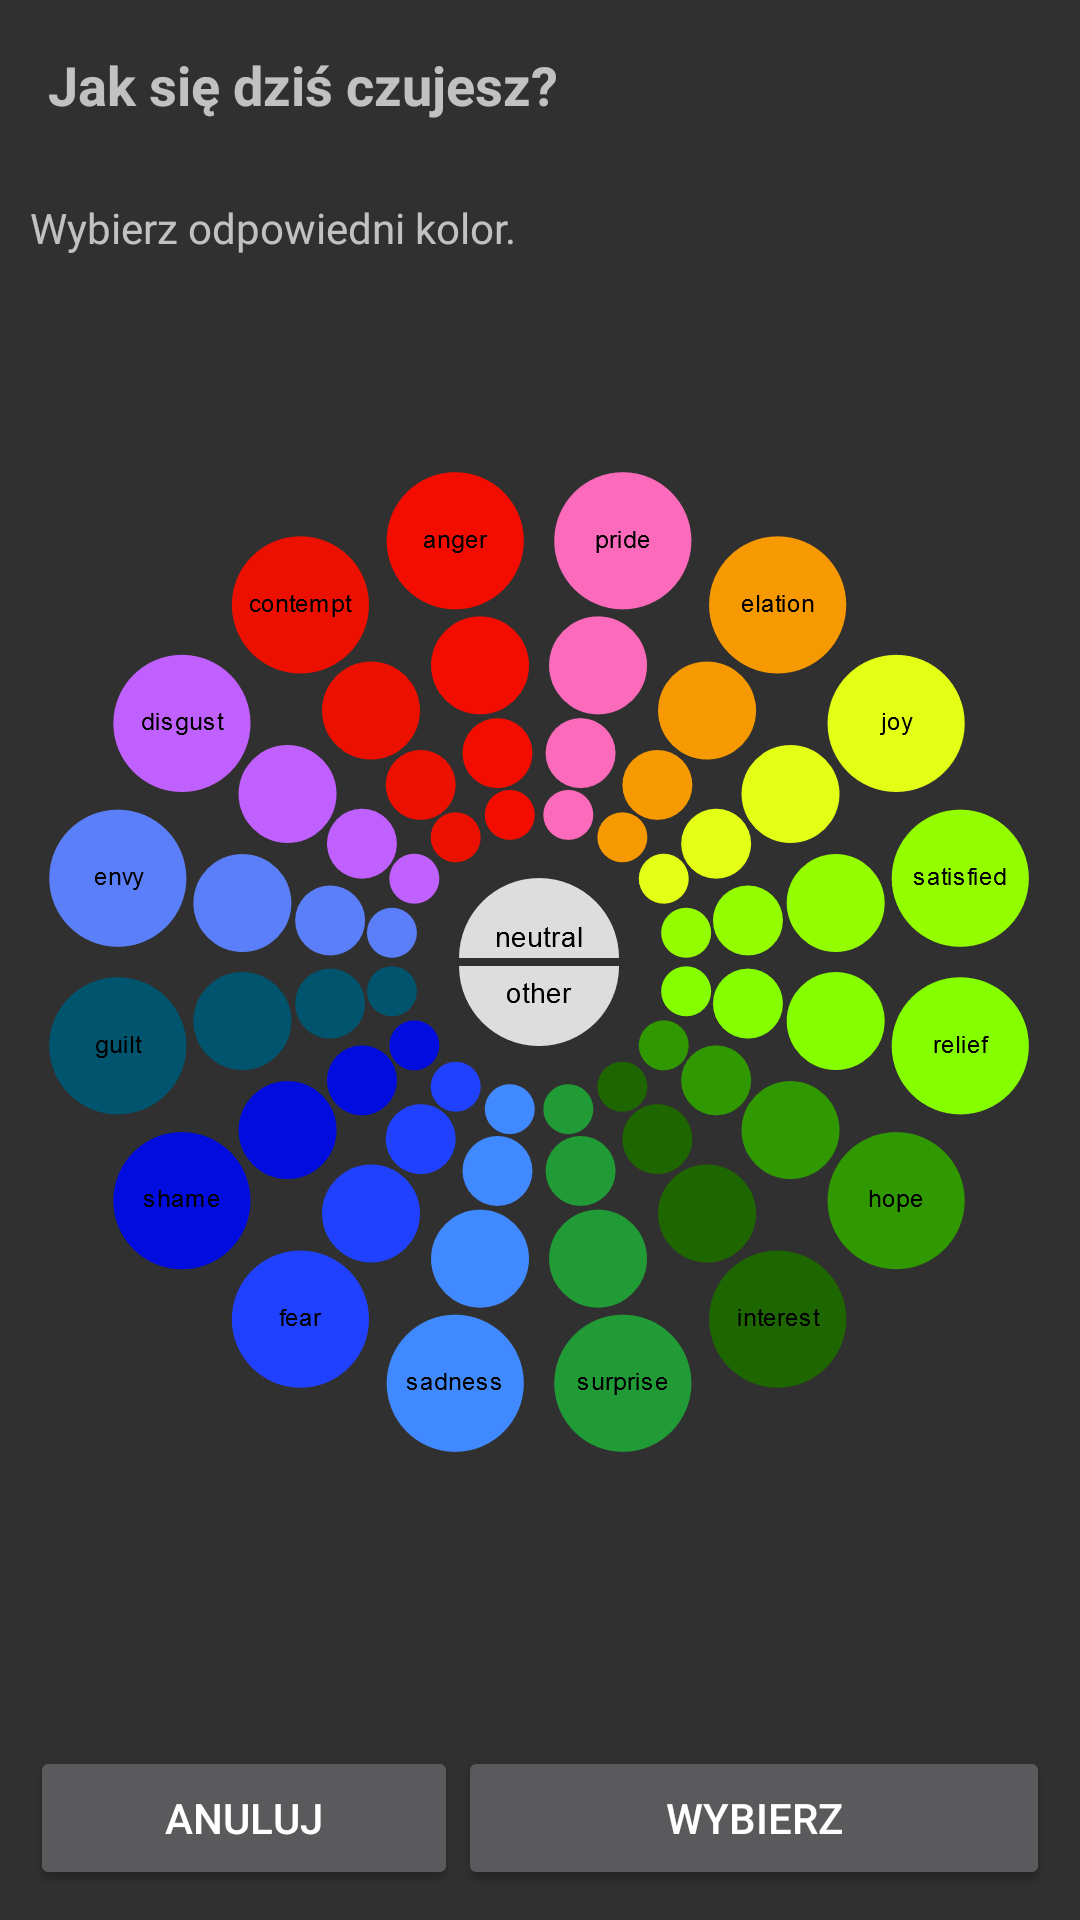
\includegraphics[scale=0.22]{rozdzial6/jspsych-geneva-wheel.png}
			\subcaption{\label{subfigure_a}}
		\end{subfigure}
		\begin{subfigure}{0.35\textwidth}
			\centering
			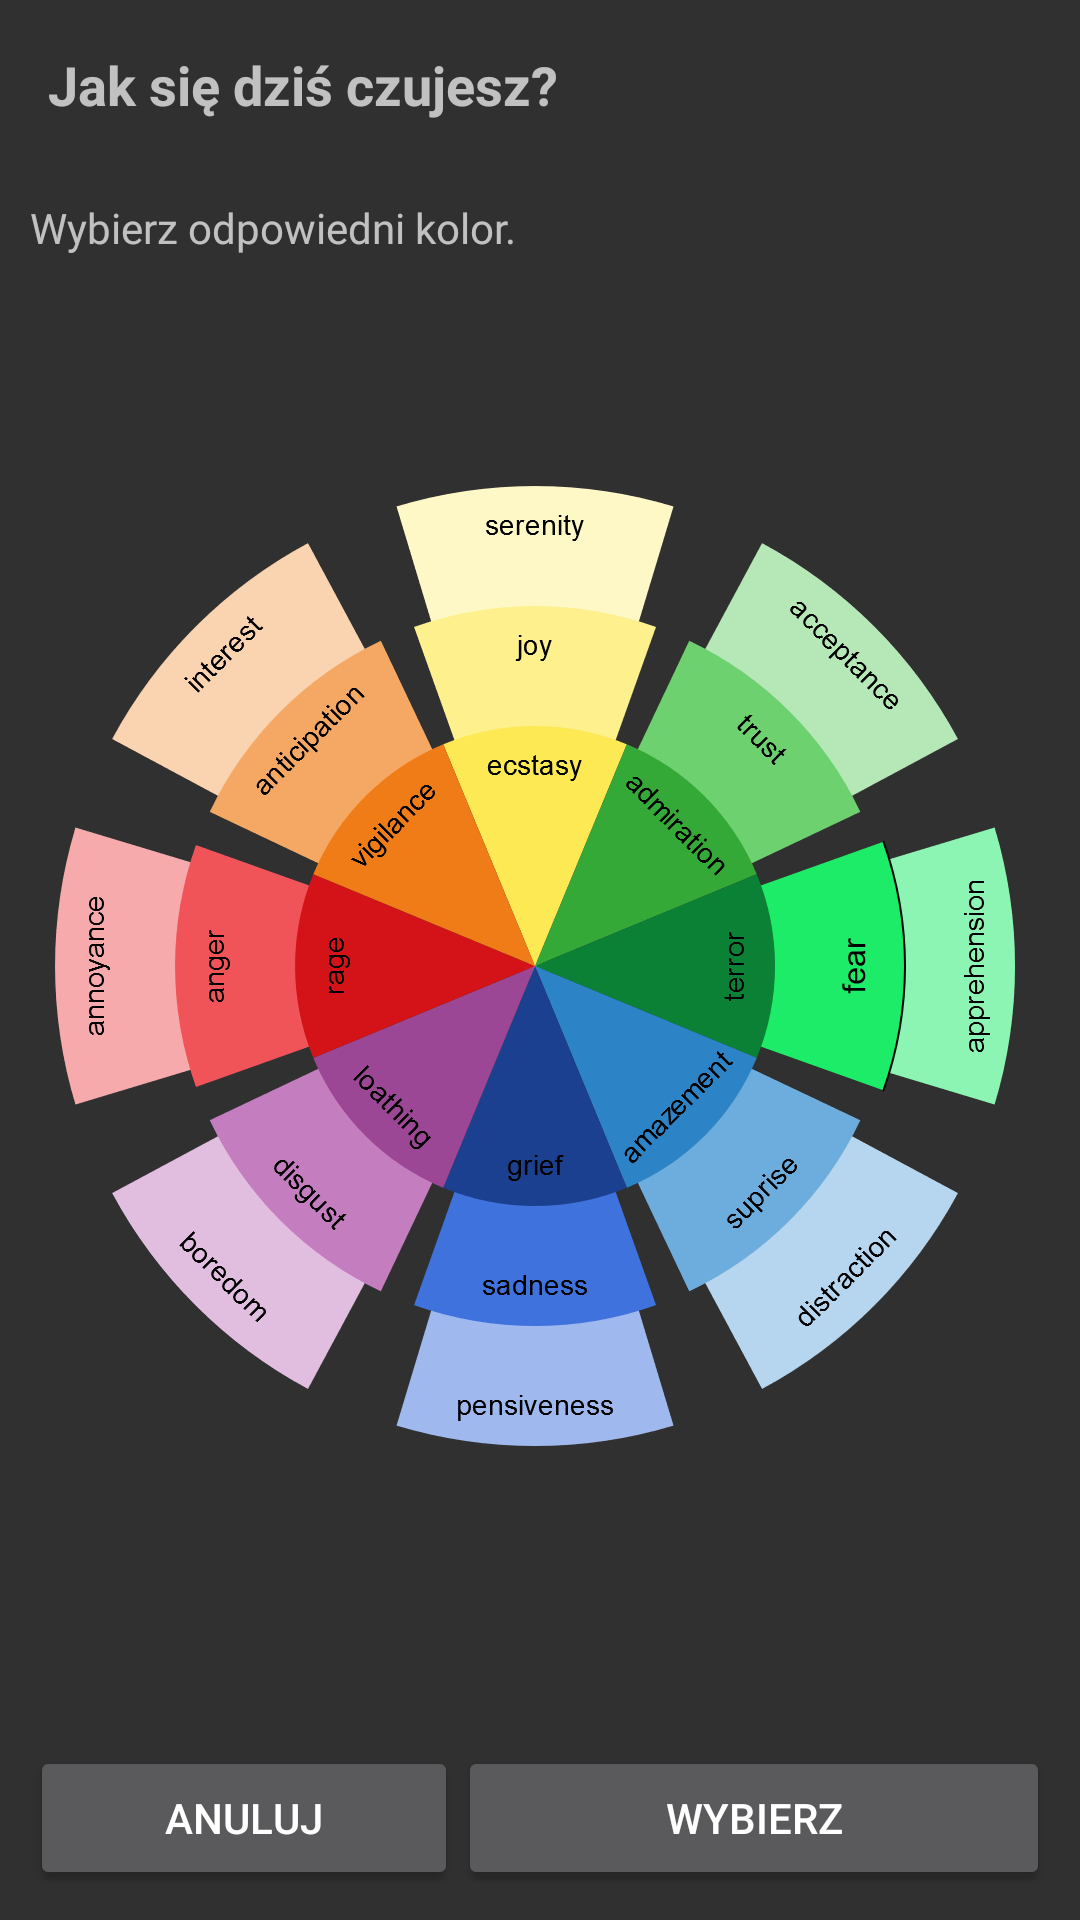
\includegraphics[scale=0.22]{rozdzial6/jspsych-plutchik-wheel-2}
			\subcaption{\label{subfigure_b}}
		\end{subfigure}
		\caption{ Zaawansowane \textit{widgety} zintegrowane z~pluginem \textit{HowAreYou: } \textit{Geneva Emotion Wheel} (a) oraz Koło Plutchika (b).}
	\end{figure}
	
\end{itemize}